\documentclass[class=scrbook, crop=false]{standalone}
\usepackage[subpreambles=true]{standalone}
\ifstandalone
    % WARNING: Proceed with caution!

% -----------------------------------------------------------------------------------
% For package standalone
% -----------------------------------------------------------------------------------
\usepackage{import}

% -----------------------------------------------------------------------------------
% Language and typeset
% -----------------------------------------------------------------------------------
\usepackage[ngerman, english]{babel}

\usepackage{subcaption}
% Umlauts and other special characters (UTF-8)
% \usepackage[utf8]{inputenc}
\usepackage{fontspec}
\setsansfont{Arial}
% \usepackage[T1]{fontenc}  % Enable accented characters and umlauts
% LuaLatex doesn't need fontenc and uses UTF-8
% \usepackage{lmodern}  % Font face


% --------------------------------------------------------------------------------
% Page formatting
% --------------------------------------------------------------------------------
% Change the header/footer for chapter beginnings and normal pages
\usepackage[automark,headsepline]{scrlayer-scrpage}

% The package provides an easy and flexible user interface to customize the page
% layout, implementing auto-centering and auto-balancing mechanisms
% WARNING: WHEN CHANGING BCOR (Binding correction), the cover needs reworking!...
\newcommand{\theBCOR}{15mm}  % Define binding correction
\usepackage[
    bindingoffset=\theBCOR,
    % showframe, % Show boxes which indicate margins and paddings
    bottom = 3.5cm, % Margins
      left = 2.5cm,
     right = 2.5cm
] {geometry}

% The package 'float' provides a container for document objects which can not be
% broken over pages, such as tables and figures
% Needed for table and figure indexes  
\usepackage{float}

% support for landscape layout
\usepackage{lscape}

% support of \tablenotes command to add notes under table
\usepackage{threeparttable}

% To allow drawing more professional tables
\usepackage{booktabs}

% --------------------------------------------------------------------------------
% Contents
% --------------------------------------------------------------------------------
% Vector graphics (for Cover page)
\usepackage{tikz} 

% Allows additional parameters when including images
\usepackage{graphicx}

% Roman font family for all headings
\addtokomafont{disposition}{\rmfamily}

% Set the line spacing to 1.5
\usepackage[onehalfspacing]{setspace}

% Improves overall text spacing
% http://www.khirevich.com/latex/microtype/
\usepackage[stretch=10]{microtype}

% Math symbols like mu outside the math environment
\usepackage{textcomp}

% A comprehensive (SI) units package∗
% For defining SI units
\usepackage[
    range-units=single,         % Formatting ranges with single unit indication: 1 - 2 m
    range-phrase=-,             % Phrase for range: 1 - 2 m vs 1 to 2 m
    separate-uncertainty=true,  % sets +- between value and uncertainty 
    multi-part-units=repeat     % In expressions with multiple values (multi part numbers) 
                                % the unit is printed each time: 1 mm x 1 mm
] {siunitx}
% https://tex.stackexchange.com/questions/124488/multi-part-numbers-and-units-in-siunitx

% Allows Sourcecodes with highlighting 
\usepackage{listings}

% This package provides user control over the layout of the three basic list
% environments: enumerate, itemize and description
\usepackage{enumitem}
\setlist{nosep} % Remove the vertical space between \item elements in all lists

% ToDo Notes
% \setlength{\marginparwidth}{2cm}
\usepackage{todonotes}
\setuptodonotes{inline, inlinepar}
\reversemarginpar  % Put ToDo notes on the binding's side
% \usepackage{soul} % Colorful ToDo notes

% Check out colors here http://latexcolor.com/
\usepackage{xcolor}

\usepackage{amsmath}    % alignment of equations

% --------------------------------------------------------------------------------
% Other elements
% --------------------------------------------------------------------------------
% Blindtext: Organic looking text dummy
\usepackage{blindtext}

% Hyperlinks within the document (PDF)
% "hidelinks" hides visual highlighting of links
\usepackage[hidelinks]{hyperref}

% Package for Glossary and Index (Acronyms are listed in a separate list) 
\usepackage[acronym, nogroupskip]{glossaries}[=v4.49] % groupskip: alphabetic grouping of entries

\usepackage{xltabular}   % <------- FOR glossaries

% Integration and management of bibliographies
\usepackage{csquotes}   % backend=biber in biblatex needs this package
\usepackage[
    style=ieee,   % style of the bibliography, entries are sorted in alphabetic order. "ieee" is another common style.
    backend=biber,      % based on package 'biber' 
    bibencoding=ascii   % ASCII Text encoding; may use "utf8" instead
] {biblatex}

% --------------------------------------------------------------------------------
%                               PATHS & FILES
% --------------------------------------------------------------------------------
% Fix paths for standalone compiling
\ifstandalone
    \def \home {..}
\else
    \def \home {.}
\fi

% Package: scrlayer-scrpage
% \def \stylePath {\home/settings+/style/page}
\input{\home/settings+/style/page}  % Load page style

% Package: graphicx
\graphicspath{{\home/images/}}  % Set path to images

% Package: listings
\input{\home/settings+/style/code.tex}  % Set path to style file
\lstset{inputpath={\home/code/}} % Default path to code listings

% Package: glossaries
\input{\home/settings+/style/symbols}  % Set path to symbols list style file
\input{\home/settings+/style/acronyms}  % Set path to acronym list style file
% -------------------------------------------------------------------------------
%               Listing of all Glossary and Acronym Entries 
%                           use as shown below
% -------------------------------------------------------------------------------

% ==== EXEMPLARY ENTRY FOR SYMBOLS LIST =========================================

% ==== EXEMPLARY ENTRY FOR ACRONYMS LIST ========================================
% \newacronym{#label}{#acronym}{#long_form}

% define new command for custom arconym entry with only two arguments
% fabricates an easier way to use \newacronym 
\newcommand{\acroX}[2]{\newacronym{#1}{#1}{#2}}
% \acroX{label and arconym}{long name}
% \acroX{CD}               {Compact Disk}

\newcommand{\acroY}[3]{\newacronym{#1}{#2}{#3}}
% \arcoY{label}{acronym}{long name}
% \acroY{CD}   {cd}     {Compact Disk}
 
\newacronym{AEP}{AEP}{Imbalance price}
\newacronym{aFRR}{aFRR}{Automatic Frequency Restoration Reserve}


\newacronym{reBAP}{reBAP}{Uniform imbalance price}
\newacronym{TSO}{TSO}{Transmission System Operator}
\newacronym{FCR}{FCR}{Frequency Containment Reserve}
\newacronym{mFRR}{mFRR}{Manual Frequency Restoration Reserve}
\newacronym{BRP}{BRP}{Balancing Responsible Party}
\newacronym{SB}{SB}{System Balance}
\newacronym{VRE}{VRE}{variable renewable energy}
\newacronym{ID1}{ID1}{intraday index ID1}
\newacronym{MAE}{MAE}{mean average error}
\newacronym{RMSE}{RMSE}{root mean squared error}
\newacronym{MSE}{MSE}{mean squared error}
\newacronym{CRPS}{CRPS}{continuous ranked probabililty score}
\newacronym{GCC}{GCC}{Grid Control Cooperation}
\newacronym{IC}{IC}{Continuous intraday}
\newacronym{VWAP}{VWAP}{volume-weighted average price}
\newacronym{VID}{VID}{traded volume within the intraday market}
\newacronym{ID AEP}{ID AEP}{Intraday Average Energy Price}
\newacronym{FRR}{FRR}{Frequency Restoration Reserve}
\newacronym{TFT}{TFT}{Temporal Fusion Transformer}
\newacronym{DLM}{DLM}{Dynamic Linear Model}
\newacronym{GB}{GB}{Gradient Boosting}
\newacronym{RF}{RF}{Random Forest}
\newacronym{ARIMAX}{ARIMAX}{Autoregressive Integrated Moving Average with eXogenous variables}
\newacronym{xLSTM}{xLSTM}{Extended Long Short-Term Memory}
\newacronym{DWD}{DWD}{Deutscher Wetterdienst}
\newacronym{ENTSO-E}{ENTSO-E}{European Network of Transmission System Operators for Electricity}
\newacronym{IDA1}{IDA1}{Intraday auction 1}
\newacronym{MOSMIX}{MOSMIX}{Model Output Statistics-MIX}
\newacronym{mLSTM}{mLSTM}{memory-optimized LSTM}
\newacronym{sLSTM}{sLSTM}{speed-optimized LSTM}

% ==== EXEMPLARY ENTRY FOR MAIN GLOSSARY ========================================

    % \newglossaryentry{policy}{name={Policy},description={Im geschäftlichen Bereich bezeichnet Policy eine interne Leit- bzw. Richtlinie, die formal durch das Unternehmen dokumentiert und über ihr Management verantwortet wird}}
    % \newglossaryentry{pcie}{name={PCI Express},description={PCI Express („Peripheral Component Interconnect Express“, abgekürzt PCIe oder PCI-E) ist ein Standard zur Verbindung von Peripheriegeräten mit dem Chipsatz eines Hauptprozessors. PCIe ist der Nachfolger von PCI, PCI-X und AGP und bietet im Vergleich zu seinen Vorgängern eine höhere Datenübertragungsrate pro Pin.}}
    % \newglossaryentry{realnumber}
  % Load glossary, symbol and acronyms list

% Package: biblatex
\addbibresource{\home/references/references.bib}  % Set path to bib resources

% Custom variables
\input{\home/settings+/variables}
% --------------------------------------------------------------------------------
%                                   OPTIONAL
% --------------------------------------------------------------------------------


% Simple arithmetic for LaTeX commands
% \usepackage{calc}

% Document Elements
% -------------------

% Index
% \usepackage{imakeidx}

% compact Lists
%\usepackage{paralist}

% visual improvements for citations
% \usepackage{epigraph}

% Create pseudo code
% https://www.overleaf.com/learn/latex/Algorithms
% \usepackage{algorithm}
% \usepackage{algorithmic}
%\usepackage[noend]{algpseudocode}

% Formatting
% -------------------
% Tweaks for scrbook, redefines commands of other packages
% \usepackage{scrhack}

% Intelligent space separator (nice for superscript?)
% \usepackage{xspace}

% Allows breaks within tables
%\usepackage{tabularx}

% Allows for page breaks in tables
% \usepackage{longtable}

% allows modifying of captions
% \usepackage{caption}

% Multiline comments
%\usepackage{verbatim}

% % Custom colors
% \definecolor{dartmouthgreen}{rgb}{0.05, 0.5, 0.06}

% IF you want to define unicode characters
% \DeclareUnicodeCharacter{0229}{\c{e}}
% \DeclareUnicodeCharacter{0306}{\u{Z}}


% Document elements
% ------------------------------------

% Table package
% \usepackage{booktabs}

% Pie diagram
% \usepackage{datapie}

% Side by Side images
% \usepackage{subcaption}

% For landscape tables
%\usepackage{pdflscape}
%\usepackage{afterpage}

% Graphics can be flow around by text
%\usepackage{wrapfig}

\fi

% ----------------------------------------------------------------------------
%                               Discussion
% ----------------------------------------------------------------------------
\begin{document}

\chapter{Results and Discussion} % Overview text
\label{Chapter::Results and Discussion}
In this chapter, the results of the thesis are discussed. The following sections contain th results of the experiments specified in \ref{Chapter::Experiments}.                   
    In this chapter, the results of the thesis are presented and evaluated as well as, the approach of this thesis.

% Show your results and analyze them
% Explain why the results are the way they are and not different
% Go into possible measurement errors and why they occurred
% Look for anomalies and explain why they occur
\section{Results}
\label{Section::Results}

\subsection{Out of the box performance}
  The results of this experiment are shown in table \ref{Table::Out_of_the_box_performance}.
  Out of the box random forest was the best at predicting the imbalance price when looking at mean average error.
  The more complex xLSTM model had better results with respect toe the RMSE. 
  When looking at the continuous ranked probability socres, ARIMA performed the best, followed closely by the iTransformer model.
  For almost all coverage percentages the native intraday ID1 index gets outperformed by all of the models.
  Here random forest performs best.
  
  \begin{table}[]
\centering
\begin{tabular}{l|l|l|l|l|l|l}
Model name 		&  RMSE 	& MAE 	& CRPS 	& 50\%-cov 	& 90\%-cov 	& 98\%-cov \\\hline
Naive intraday ID1 	& 308.69 	& 93.17 	& 42.90 	& 0.08 		& 0.56 		& 0.84 \\
Random forest 		& 241.37	&   \underline{90.22} 	& 52.38 	& 0.32 		& 0.80 		& 0.94 \\
Arima 			& 358.75 	& 100.5 	& 42.04  	& 0.21 		& 0.61 		& 0.81 \\	
iTransformer 		& 367.50 	& 111.66 	& 42.40 	& 0.09 		& 0.66 		& 0.84 \\
xLSTM 			&  \underline{156.40} 	& 107.65 	& 51.41 	& 0.25 		& 0.68 		& 0.84 \\
\end{tabular}
\caption{Out of the box performance for all models}
\label{Table::Out_of_the_box_performance}
\end{table}


\begin{figure}
  \centering
\begin{subfigure}{0.45\textwidth}
  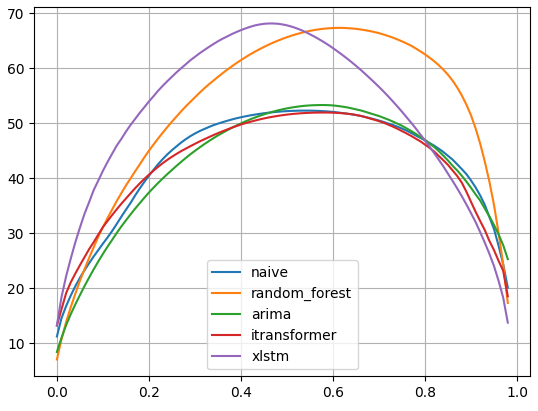
\includegraphics[width=\linewidth]{../images/results/quantile_pinball_scores.png}
  \caption{Quantile pinball scores for all models}
\end{subfigure}
\begin{subfigure}{0.45\textwidth}
  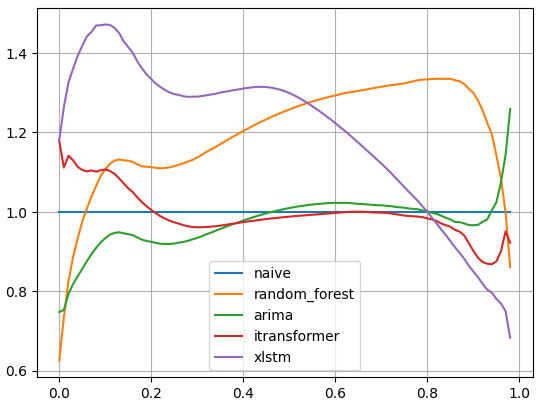
\includegraphics[width=\linewidth]{../images/results/quantile_pinball_scores_to_id1.png}
  \caption{Quantile pinball scores normalized based on naive}
\end{subfigure}
\caption{Quantile pinball scores for each model}
\label{Figure::pinball_scores}
\end{figure}


Figure \ref{Figure::pinball_scores} shows the pinball scores for each quantile for each model.
On the left the raw pinball scores are shown.
The right graph shows the pinball score in relation to the pinball score of the naive model.
These values are calculated by dividing the pinball score for each quantile $q$ for each model by the the pinball score for the quantile $q$ for the naive model.

These charts show, that random forest performs the best on the lowest quantile and is among the best in the higher quantiles. 
Across most of the percentiles, from about $0.1$ to $0.8$ both random forest and xlstm have the worst pinball score.
The xLSTM shines in the higher quantiles. 
The pinball scores for xLSTM are the best in the higher percentiles. 
This is in line with this model having the best RMSE, due to the nature of the otliers being very extreme.


Figure \ref{Figure::Model_predictions} shows the predictions for the machine learning models on an example day and the actual imbalance price.

\begin{figure}
  \centering
\begin{subfigure}{0.45\textwidth}
  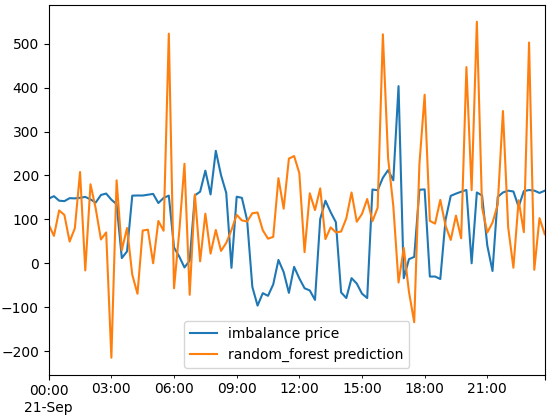
\includegraphics[width=\linewidth]{../images/results/random_forest_prediction.png}
  \caption{Predictions of random forest}
\end{subfigure}
\begin{subfigure}{0.45\textwidth}
  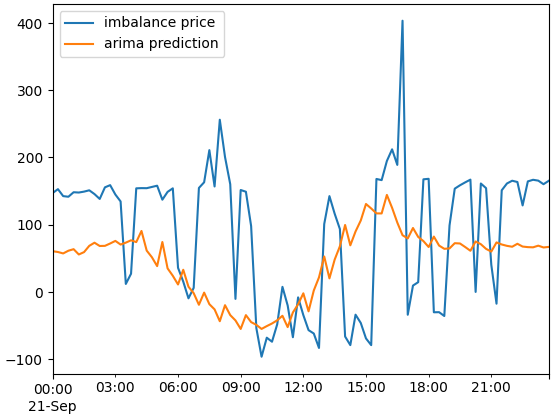
\includegraphics[width=\linewidth]{../images/results/arima_prediction.png}
  \caption{Predictions of ARIMA}
\end{subfigure}
\begin{subfigure}{0.45\textwidth}
  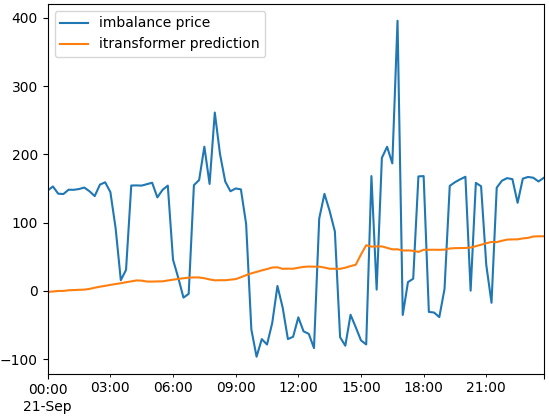
\includegraphics[width=\linewidth]{../images/results/itransformer_prediction.png}
  \caption{Predictions of iTransformer}
\end{subfigure}
\begin{subfigure}{0.45\textwidth}
  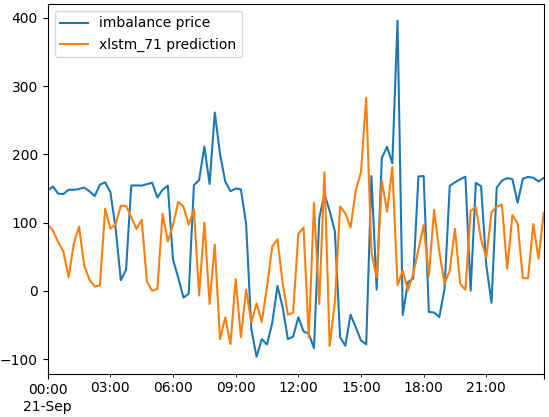
\includegraphics[width=\linewidth]{../images/results/xlstm_prediction.png}
  \caption{Predictions of xLSTM}
\end{subfigure}
\caption{Predictions of the different models on example day}
\label{Figure::Model_predictions}
\end{figure}

While random forest better predicticts the imbalance price with regards to mean average error, the xLSTM model seems to better capture outlieres, resulting in a lower mean squared error.


\subsection{Different xLSTM block structures}

  \begin{table}[]
\centering
\begin{tabular}{l|l|l|l|l|l|l}
Configuration name &  RMSE & MAE & CRPS & 50\%-cov & 90\%-cov & 98\%-cov \\\hline
xLSTM\_1\_0 & 154.87 & 109.50& 50.45& 0.30 & 0.76 & 0.87 \\
xLSTM\_0\_1& 152.82 & 107.81 & 51.00 & 0.25 & 0.76 & 0.89 \\
xLSTM\_7\_1 & 156.40 & 107.65 & 51.41 & 0.25 & 0.68 & 0.84 \\
\end{tabular}
\caption{Performance for different xLSTM block configurations}
\label{Table::Performance_xLSTM}
\end{table}

Using different xLSTM configuration did not significantly increase the performance of the xLSTM model.

\subsection{iTransformer variable sequence length}

The results for this experiments can be found in table \ref{Table::Performane_sequence_length}.
The mean average error and root mean squared error does not increase or decrease with increased or decreased sequence length.
While both of these error metrics stay about the same, the quantile predictions for a sequence length of 384 is worse than the other two sequence lenghts.
 \begin{table}[]
\centering
\begin{tabular}{l|l|l|l|l|l|l}
 Configuration name &  RMSE & MAE & CRPS & 50\%-cov & 90\%-cov & 98\%-cov \\\hline
 iTransformer 96 seq & 367.50 & 111.66 & 42.40&0.09 & 0.66 & 0.84 \\
 iTransformer 192 seq & 368.45 &114.67& 43.07& 0.08 & 0.60	 & 0.83 \\
 iTransformer 384 seq & 362.46 & 107.08& 44.17	& 0.06	 &0.42	 & 0.84\\
\end{tabular}
\caption{iTransformer performance for different sequence lengths}
\label{Table::Performance_sequence_length}
\end{table}

Figure \ref{Result::iTransformer_sequence_length} shows predictions of the models trained with different sequence lengths on an example day.
The predictions of the models trained on longe sequence lengths look more like a straight line, while the model trained with the shortest sequence length has more fluctuations.

\begin{figure}
  \centering
  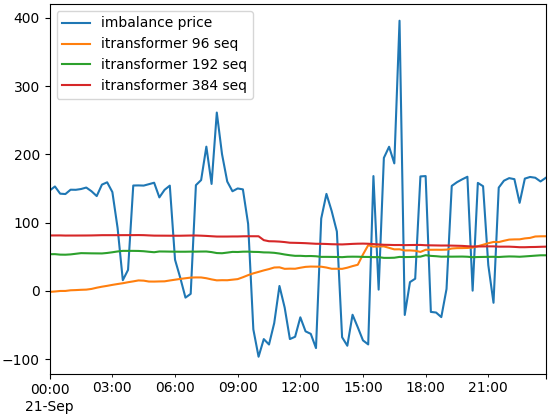
\includegraphics[width=.8\linewidth]{../images/results/itransformer_sequence_length_results.png}
  \caption{Predictions of iTransformers with different sequence lengths}
\label{Result::iTransformer_sequence_length}
\end{figure}

\subsection{iTransformer multiple target variables}

The models trained on multiple target variables performed almost identically.
The results for this experiment can be found in \ref{Table::Performance_targets}.
Figure \ref{Figure::Targets_prediction} shows the prediction of the models on an example day.
The chart on the left compares the predictions to the actual imbalance price while the chart on the right only compares the predictions with each other to magnify differences.

The predictions are almost identical, the inclusion of multiple target variables had no improving effect on the prediction of the imbalance price.

 \begin{table}[]
\centering
\begin{tabular}{l|l|l|l|l|l|l}
 Configuration name			&  RMSE 	& MAE 	& CRPS 	& 50\%-cov & 90\%-cov & 98\%-cov \\\hline
 iTransformer intraday indices 		& 367.32	&111.52	&42.40	&0.09			& 0.66	 & 0.84 \\
 iTransformer entsoe data		&  367.89	& 111.98 	&42.39	&0.09			& 0.66	 &0.83 \\
 iTransformer netzregelverbund 	& 367.55 	& 111.70	& 42.40	&0.09		 &0.66	 & 0.83\\
 iTransformer combined 		& 367.21 	& 111.42	& 42.40	& 0.10	 &0.66	 & 0.84\\
\end{tabular}
\caption{iTransformer performance for multiple target variables}
\label{Table::Performance_targets}
\end{table}


\begin{figure}
  \centering
\begin{subfigure}{0.45\textwidth}
  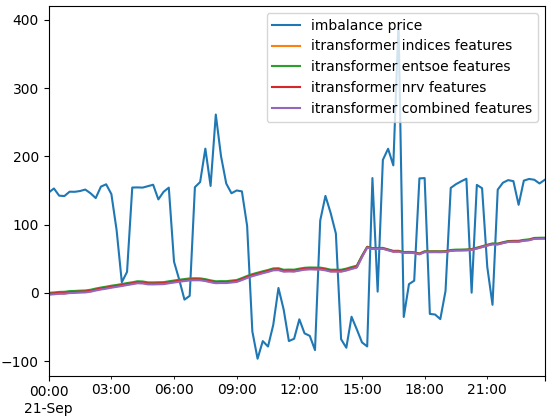
\includegraphics[width=\linewidth]{../images/results/itransformer_target_variables_aep.png}
  \caption{Predictions of models with imbalance price}
\end{subfigure}
\begin{subfigure}{0.45\textwidth}
  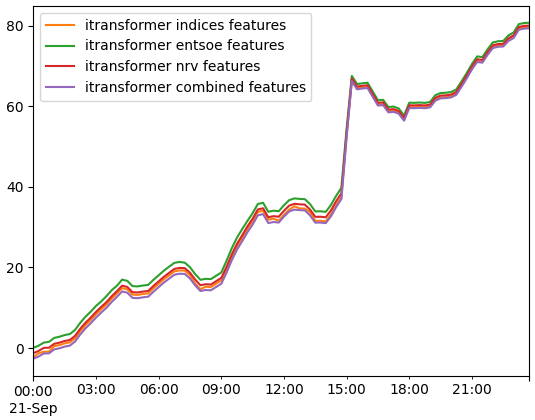
\includegraphics[width=\linewidth]{../images/results/itransformer_target_variables_alone.png}
  \caption{Predictions of models without imbalance price}
\end{subfigure}
\caption{Predictions of iTransformers trained on multiple target variables}
\label{Figure::Targets_prediction}
\end{figure}


\subsection{iTransformer different prediction horizons}


 \begin{table}[]
\centering
\begin{tabular}{l|l|l|l|l|l|l}
 Configuration name			&  RMSE 	& MAE 	& CRPS 	& 50\%-cov & 90\%-cov & 98\%-cov \\\hline
 iTransformer 4 horizon			& 364.65	&108.98	&42.55	&0.12		& 0.64	 & 0.85 \\
 iTransformer 12 horizon			& 364.69	&108.93	&42.55	&0.12		& 0.63	 & 0.85 \\
 iTransformer 24 horizon			& 364.23	&108.26	&42.67	&0.13		& 0.60	 &0.85 \\
 iTransformer 48 horizon			& 367.78	&111.51	&42.39	&0.09		& 0.66	 & 0.84 \\
 iTransformer 96 horizon			& 368.28	&111.68	&42.45	&0.09		& 0.66	 & 0.84 \\
\end{tabular}
\caption{iTransformer performance for multiple target variables}
\label{Table::Performance_targets}
\end{table}

\begin{figure}
  \centering
\begin{subfigure}{0.45\textwidth}
  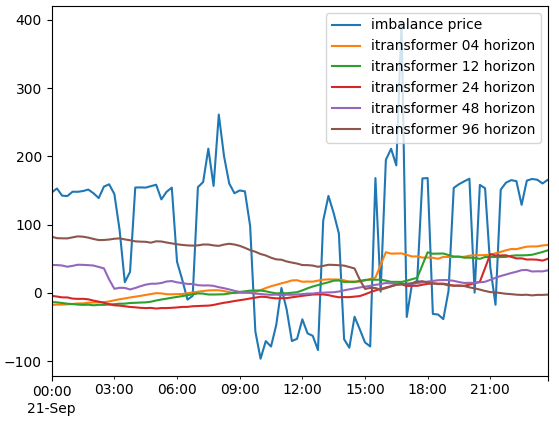
\includegraphics[width=\linewidth]{../images/results/itransformer_horizon_lengths.png}
  \caption{Predictions of models with imbalance price}
\end{subfigure}
\begin{subfigure}{0.45\textwidth}
  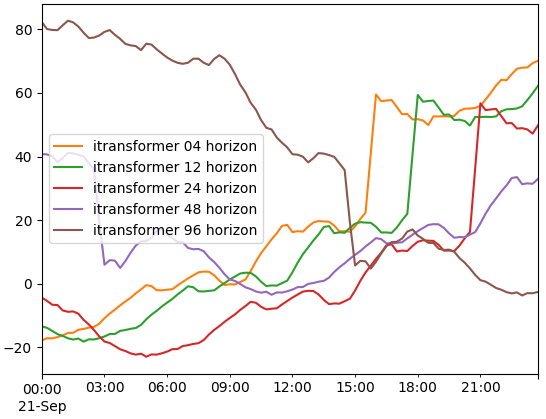
\includegraphics[width=\linewidth]{../images/results/itransformer_horizon_lengths_alone.png}
  \caption{Predictions of models without imbalance price}
\end{subfigure}
\caption{Predictions of iTransformers trained on different forecasting horizons}
\label{fig:fig}
\end{figure}


\section{Analysis or Evaluation of Something}
\label{Section::Analysis or Evaluation of Something}    

Table \ref{Table::Feature_importance} contains information about the most important features for the random forest prediction.
The top 6 most important features consist of information about prices. Interesting is, that the intraday index shifted by one day still has a very high feature importance.
The next two most important features \textit{lignite actual generation shifted by 30 minuts} and \textit{fossil hard coal actual generation shifted 30 minutes} contain information about generated energy provided by fossil energy sources.
The third features containing information about fossil energy sources ranks 14\textsuperscript{th} most important. 
The importance of features doesn't change much after the  10\textsuperscript{th} most important feature.
Out of the wheather data the temperature was the most important, followed by the difference in forecast for the solar radiation within one hour.
Notable information from this importance is that the forecasted residual load is more important to the model than the shifted actual residual load or the shifted forecasting error.
For solar and wind offshore generation the opposite is true. 
The shifted forecasting error is more important than both the forecast and the shifted actual measurement.

\begin{table}[]
\centering
\begin{tabular}{l|l|l}
 \# & Parameter & Importance \\\hline
 1 & Hourly spot price& 0.0157\\
 2 & IDA1&0.0142 \\
 3 &Aep schaetzer shifted 30 minutes&0.0081 \\
 4 & intraday ID1 shifted 1 day &0.0081\\
 5 &intraday ID3 shifted 1 day &0.0066\\
 6 &intraday IDFULL shifted 1 day &0.0055\\
 7 &lignite actual generation shifted 30 minutes&0.0035 \\
 8&fossil hard coal actual generation shifted 30 minutes &0.0034\\
 9&forecasted residual load &0.0029\\
 10&stundenwert der feuchttemperatur shifted 1 hour &0.0026\\
 11&activated srl shifted 30 minutes&0.0026 \\
 12&nrv saldo shifted 30 minutes &  0.0025\\
 13&Diff\_Rad1h&0.0025 \\
14& fossil gas actual generation shifted 30 minutes&0.0023 \\
15&hydro pumped storage actual generation shifted 30 minutes&0.0023\\
16&hourly sum for long wave atmospheric radiation shifted 1 hour&0.0022 \\
17&solar forecasting error shifted 30 minutes &0.0021\\
18&wind offshore forecasting error shifted 30 minutes&0.0021 \\
19&activated srl shifted 30 minutes&0.0020 \\
20&wind onshore actual generation shifted 30 minutes &0.0020\\
\end{tabular}
\caption{20 most important features of random forest sorted from most important to least important. Shifted features are excluded for this ranking.}
\label{Table::Feature_importance}
\end{table}


\end{document}
